% Options for packages loaded elsewhere
% Options for packages loaded elsewhere
\PassOptionsToPackage{unicode}{hyperref}
\PassOptionsToPackage{hyphens}{url}
%
\documentclass[
  ignorenonframetext,
  aspectratio=169,
]{beamer}
\newif\ifbibliography
\usepackage{pgfpages}
\setbeamertemplate{caption}[numbered]
\setbeamertemplate{caption label separator}{: }
\setbeamercolor{caption name}{fg=normal text.fg}
\beamertemplatenavigationsymbolsempty
% remove section numbering
\setbeamertemplate{part page}{
  \centering
  \begin{beamercolorbox}[sep=16pt,center]{part title}
    \usebeamerfont{part title}\insertpart\par
  \end{beamercolorbox}
}
\setbeamertemplate{section page}{
  \centering
  \begin{beamercolorbox}[sep=12pt,center]{section title}
    \usebeamerfont{section title}\insertsection\par
  \end{beamercolorbox}
}
\setbeamertemplate{subsection page}{
  \centering
  \begin{beamercolorbox}[sep=8pt,center]{subsection title}
    \usebeamerfont{subsection title}\insertsubsection\par
  \end{beamercolorbox}
}
% Prevent slide breaks in the middle of a paragraph
\widowpenalties 1 10000
\raggedbottom
\usepackage{iftex}
\ifPDFTeX
  \usepackage[T1]{fontenc}
  \usepackage[utf8]{inputenc}
  \usepackage{textcomp} % provide euro and other symbols
\else % if luatex or xetex
  \usepackage{unicode-math} % this also loads fontspec
  \defaultfontfeatures{Scale=MatchLowercase}
  \defaultfontfeatures[\rmfamily]{Ligatures=TeX,Scale=1}
\fi
\usepackage{lmodern}

\usetheme[]{metropolis}
\ifPDFTeX\else
  % xetex/luatex font selection
\fi
% Use upquote if available, for straight quotes in verbatim environments
\IfFileExists{upquote.sty}{\usepackage{upquote}}{}
\IfFileExists{microtype.sty}{% use microtype if available
  \usepackage[]{microtype}
  \UseMicrotypeSet[protrusion]{basicmath} % disable protrusion for tt fonts
}{}
\makeatletter
\@ifundefined{KOMAClassName}{% if non-KOMA class
  \IfFileExists{parskip.sty}{%
    \usepackage{parskip}
  }{% else
    \setlength{\parindent}{0pt}
    \setlength{\parskip}{6pt plus 2pt minus 1pt}}
}{% if KOMA class
  \KOMAoptions{parskip=half}}
\makeatother


\usepackage{longtable,booktabs,array}
\usepackage{calc} % for calculating minipage widths
\usepackage{caption}
% Make caption package work with longtable
\makeatletter
\def\fnum@table{\tablename~\thetable}
\makeatother
\usepackage{graphicx}
\makeatletter
\newsavebox\pandoc@box
\newcommand*\pandocbounded[1]{% scales image to fit in text height/width
  \sbox\pandoc@box{#1}%
  \Gscale@div\@tempa{\textheight}{\dimexpr\ht\pandoc@box+\dp\pandoc@box\relax}%
  \Gscale@div\@tempb{\linewidth}{\wd\pandoc@box}%
  \ifdim\@tempb\p@<\@tempa\p@\let\@tempa\@tempb\fi% select the smaller of both
  \ifdim\@tempa\p@<\p@\scalebox{\@tempa}{\usebox\pandoc@box}%
  \else\usebox{\pandoc@box}%
  \fi%
}
% Set default figure placement to htbp
\def\fps@figure{htbp}
\makeatother





\setlength{\emergencystretch}{3em} % prevent overfull lines

\providecommand{\tightlist}{%
  \setlength{\itemsep}{0pt}\setlength{\parskip}{0pt}}



 


% ============================================================
%  ECO 2203 — Beamer Metropolis Theme Preamble
%  Course: International Trade and Policy in Agriculture
%  Instructor: Nithin M, Department of Development Economics
% ============================================================

% MUST be first: load Metropolis theme before \metroset and colour overrides
\usetheme{metropolis}

% Only load packages not already provided by pandoc's beamer template
\usepackage{amsmath,amssymb}

% ---- Brand colours -----------------------------------------
\definecolor{brandblue}{HTML}{012169}
\definecolor{brandgold}{HTML}{B9975B}
\definecolor{lightblue}{HTML}{E8EDF5}

% ---- Metropolis colour overrides ---------------------------
% Main palette
\setbeamercolor{normal text}{fg=black,bg=white}
\setbeamercolor{alerted text}{fg=brandgold}
\setbeamercolor{example text}{fg=brandblue!70!black}

% Title slide
\setbeamercolor{title}{fg=white,bg=brandblue}
\setbeamercolor{subtitle}{fg=brandgold}
\setbeamercolor{author}{fg=white}
\setbeamercolor{institute}{fg=brandgold!80!white}
\setbeamercolor{date}{fg=white}
\setbeamercolor{title page header}{fg=white,bg=brandblue}

% Frametitle bar
\setbeamercolor{frametitle}{fg=white,bg=brandblue}

% Progress bar → gold
\setbeamercolor{progress bar}{fg=brandgold,bg=brandblue!30}
\setbeamercolor{title separator}{fg=brandgold}
\setbeamercolor{progress bar in head/foot}{fg=brandgold,bg=brandblue!20}
\setbeamercolor{progress bar in section page}{fg=brandgold,bg=brandblue!20}

% Blocks
\setbeamercolor{block title}{bg=brandblue,fg=white}
\setbeamercolor{block body}{bg=lightblue,fg=black}
\setbeamercolor{block title alerted}{bg=brandgold,fg=white}
\setbeamercolor{block body alerted}{bg=brandgold!12,fg=black}
\setbeamercolor{block title example}{bg=brandblue!70!black,fg=white}
\setbeamercolor{block body example}{bg=brandblue!8,fg=black}

% Structure / lists
\setbeamercolor{structure}{fg=brandblue}
\setbeamercolor{section in toc}{fg=brandblue}
\setbeamercolor{itemize item}{fg=brandblue}
\setbeamercolor{itemize subitem}{fg=brandgold}
\setbeamercolor{enumerate item}{fg=brandblue}
\setbeamercolor{description item}{fg=brandblue}

% ---- Metropolis options ------------------------------------
\metroset{
  progressbar    = frametitle,   % gold bar under frametitle
  sectionpage    = none,
  numbering      = fraction,
  block          = fill
}

% ---- Fonts (Metropolis uses Fira Sans; fallback gracefully) -
\setbeamerfont{title}{size=\Large,series=\bfseries}
\setbeamerfont{subtitle}{size=\normalsize,series=\mdseries}
\setbeamerfont{frametitle}{size=\large,series=\bfseries}
\setbeamerfont{block title}{size=\normalsize,series=\bfseries}
\setbeamerfont{caption}{size=\footnotesize}

% ---- Footer: course info + slide number --------------------
\setbeamertemplate{footline}{%
  \begin{beamercolorbox}[wd=\paperwidth,ht=2.0ex,dp=1ex]{footline}%
    \hspace{0.8em}%
    {\footnotesize\color{brandblue!60}%
      ECO 2203 \textbar{} International Trade and Policy in Agriculture
      \hfill Nithin M \hfill
      \insertframenumber{}/\inserttotalframenumber\hspace{0.8em}}%
  \end{beamercolorbox}%
}

% ---- Misc --------------------------------------------------
\setlength{\parskip}{0.25em}
\setbeamertemplate{navigation symbols}{}

% tighter column sep for side-by-side content
\setlength{\columnsep}{0.8em}

% Fix: make \label truly robust in moving arguments (Quarto generates
% \caption{\label{fig-xxx}...} which crashes Metropolis in batchmode).
% DeclareRobustCommand creates a self-protecting robust version.
\makeatletter
\let\quarto@originallabel\label
\DeclareRobustCommand*{\label}[1]{\quarto@originallabel{#1}}
\makeatother

% Prevent figures from overflowing Beamer frames.
% width=\linewidth: scale to text width (already Quarto default);
% height=0.6\textheight: cap height so figures never push past the frame bottom.
% keepaspectratio: never distort — whichever constraint binds first wins.
\setkeys{Gin}{width=\linewidth,height=0.6\textheight,keepaspectratio}
\makeatletter
\@ifpackageloaded{caption}{}{\usepackage{caption}}
\AtBeginDocument{%
\ifdefined\contentsname
  \renewcommand*\contentsname{Table of contents}
\else
  \newcommand\contentsname{Table of contents}
\fi
\ifdefined\listfigurename
  \renewcommand*\listfigurename{List of Figures}
\else
  \newcommand\listfigurename{List of Figures}
\fi
\ifdefined\listtablename
  \renewcommand*\listtablename{List of Tables}
\else
  \newcommand\listtablename{List of Tables}
\fi
\ifdefined\figurename
  \renewcommand*\figurename{Figure}
\else
  \newcommand\figurename{Figure}
\fi
\ifdefined\tablename
  \renewcommand*\tablename{Table}
\else
  \newcommand\tablename{Table}
\fi
}
\@ifpackageloaded{float}{}{\usepackage{float}}
\floatstyle{ruled}
\@ifundefined{c@chapter}{\newfloat{codelisting}{h}{lop}}{\newfloat{codelisting}{h}{lop}[chapter]}
\floatname{codelisting}{Listing}
\newcommand*\listoflistings{\listof{codelisting}{List of Listings}}
\makeatother
\makeatletter
\makeatother
\makeatletter
\@ifpackageloaded{caption}{}{\usepackage{caption}}
\@ifpackageloaded{subcaption}{}{\usepackage{subcaption}}
\makeatother

\usepackage{bookmark}
\IfFileExists{xurl.sty}{\usepackage{xurl}}{} % add URL line breaks if available
\urlstyle{same}
\hypersetup{
  pdftitle={Terms of Trade, Free Trade \& Free Trade Agreements},
  pdfauthor={Nithin M},
  hidelinks,
  pdfcreator={LaTeX via pandoc}}


\title{Terms of Trade, Free Trade \& Free Trade Agreements}
\subtitle{ECO 2203 \textbar{} International Trade and Policy in
Agriculture}
\author{Nithin M}
\date{2026-05-30}
\institute{Department of Development Economics}

\begin{document}
\frame{\titlepage}


\section{Part I: Terms of Trade}\label{part-i-terms-of-trade}

\begin{frame}{Recap: From Theory to Exchange}
\phantomsection\label{recap-from-theory-to-exchange}
\begin{columns}[T]
\begin{column}{0.6\linewidth}
\textbf{The journey so far:}

\begin{longtable}[]{@{}ll@{}}
\toprule\noalign{}
Theory & Core Insight \\
\midrule\noalign{}
\endhead
Mercantilism & Accumulate gold via export surplus \\
Absolute Advantage & Export what you produce more efficiently \\
Comparative Advantage & Export where opportunity cost is lower \\
Heckscher-Ohlin & Export goods intensive in your abundant factor \\
Lewis Model & Surplus labour enables low-cost production \\
\bottomrule\noalign{}
\end{longtable}

\textbf{What these theories explain:} \emph{What} countries trade and
\emph{why.}

\textbf{What they don't fully answer:}

\begin{quote}
At \emph{what price} do countries exchange their exports and imports?
And are these prices moving in India's favour?
\end{quote}

\textbf{→ Terms of Trade}
\end{column}

\begin{column}{0.4\linewidth}
\textbf{Why terms of trade matter:}

Two countries can both have comparative advantage-based trade --- but if
one country's export prices are falling relative to its import prices,
it may be getting poorer even as trade volume grows.

This is the core concern of the \textbf{Prebisch-Singer Hypothesis} ---
and it has profound implications for India's agricultural sector.
\end{column}
\end{columns}
\end{frame}

\begin{frame}{What Are Terms of Trade?}
\phantomsection\label{what-are-terms-of-trade}
\textbf{Definition: Terms of Trade}

The rate at which a country's exports exchange for its imports in
international markets.

\emph{``How many units of imports can I buy with one unit of exports?''}

\begin{columns}[T]
\begin{column}{0.5\linewidth}
\textbf{Commodity (Net Barter) Terms of Trade:}

\[ToT = \frac{P_X}{P_M} \times 100\]

Where \(P_X\) = export price index; \(P_M\) = import price index.

\textbf{Interpretation:} - ToT = 100 → base year benchmark - ToT
\textgreater{} 100 → terms \emph{improved} (exports buy more imports) -
ToT \textless{} 100 → terms \emph{worsened} (exports buy fewer imports)
\end{column}

\begin{column}{0.5\linewidth}
\textbf{Other ToT Measures:}

\textbf{Gross Barter ToT:} \[= \frac{Q_M}{Q_X}\] (Physical quantity
ratio of imports to exports)

\textbf{Income ToT:} \[= \frac{P_X \times Q_X}{P_M}\] (Export revenue /
import price --- measures import capacity)

\textbf{Single Factoral ToT:} \[= ToT \times Z_X\] (Adjusts for export
sector productivity \(Z_X\))

For India's agricultural policy analysis, we primarily use the
\textbf{commodity ToT}.
\end{column}
\end{columns}
\end{frame}

\begin{frame}{Offer Curves: Deriving the Equilibrium Terms of Trade}
\phantomsection\label{offer-curves-deriving-the-equilibrium-terms-of-trade}
\textbf{Offer Curve (Salvatore, Ch. 4):} Shows the quantity of its
export good a nation is \emph{willing to offer} at each terms of trade,
in exchange for imports.

For each possible ToT ratio \(\tau = P_X / P_M\), the offer curve traces
the export-import combination a country would choose given its
preferences and PPF:

\[\text{Nation offers } X(\tau) \text{ exports to obtain } M(\tau) \text{ imports at terms } \tau\]

\begin{itemize}
\tightlist
\item
  As ToT improves (each unit of exports buys more imports), a nation
  offers more exports
\item
  \textbf{Equilibrium ToT} is determined by the \emph{intersection} of
  the two nations' offer curves
\item
  Stability: any deviation from \(E^*\) creates excess supply/demand
  that restores equilibrium
\end{itemize}

\begin{figure}

\centering{

\pandocbounded{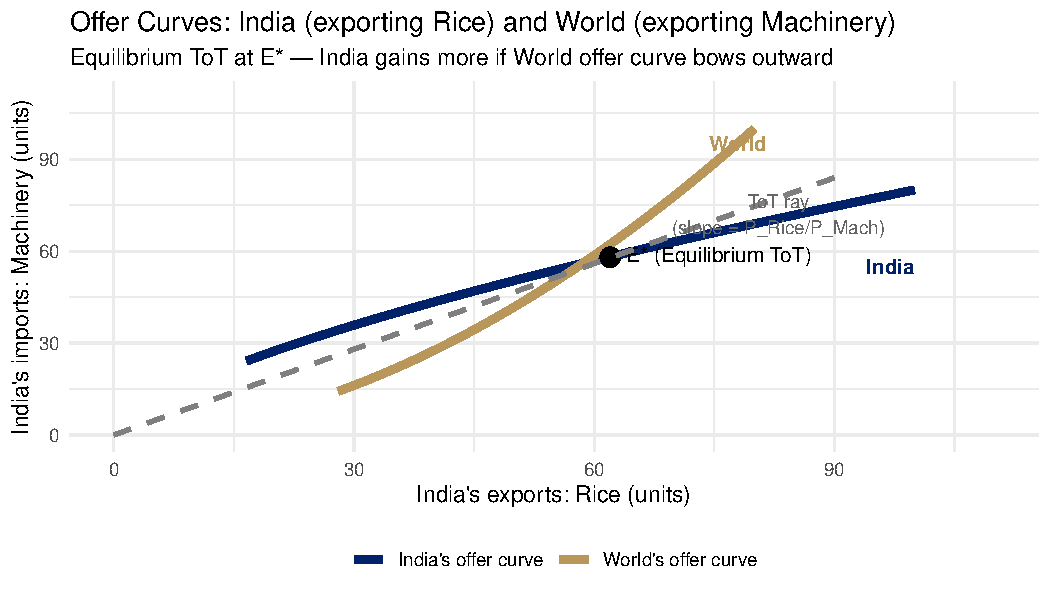
\includegraphics[keepaspectratio]{Lecture06_Terms_of_Trade_files/figure-beamer/fig-offer-curves-1.pdf}}

}

\caption{\label{fig-offer-curves}Offer Curves: Equilibrium Terms of
Trade Between India (Rice) and World (Machinery) Source: Author's
illustration.}

\end{figure}%

\textbf{Key insight (Salvatore Ch. 4):} The more inelastic a country's
offer curve, the greater its terms-of-trade gain. India's bargaining
power in trade improves when its exports are hard to substitute globally
(e.g., Basmati rice, specific spices).
\end{frame}

\begin{frame}{Calculating Terms of Trade: Numerical Example}
\phantomsection\label{calculating-terms-of-trade-numerical-example}
\textbf{Scenario:} India exports rice, imports petroleum.

\begin{columns}[T]
\begin{column}{0.55\linewidth}
\textbf{Base Year (FY2020):}

\begin{itemize}
\tightlist
\item
  Rice price: \textbf{\$400/tonne} → index = 100
\item
  Petroleum price: \textbf{\$60/barrel} → index = 100
\item
  \textbf{ToT = 100/100 × 100 = 100}
\end{itemize}

\begin{center}\rule{0.5\linewidth}{0.5pt}\end{center}

\textbf{Case 1: Rice price rises to \$480/tonne (FY2021)}

\begin{itemize}
\tightlist
\item
  Rice index = 120; Petroleum index = 100
\item
  \textbf{ToT = 120/100 × 100 = 120} → \emph{Terms improved}
\item
  India can now buy 20\% more oil per tonne of rice exported
\end{itemize}

\begin{center}\rule{0.5\linewidth}{0.5pt}\end{center}

\textbf{Case 2: Oil price rises to \$90/barrel (FY2022)}

\begin{itemize}
\tightlist
\item
  Rice index = 120; Petroleum index = 150
\item
  \textbf{ToT = 120/150 × 100 = 80} → \emph{Terms worsened}
\item
  India gets fewer barrels of oil per tonne of rice
\end{itemize}
\end{column}

\begin{column}{0.45\linewidth}
\textbf{FY2022 was exactly this scenario:}

\begin{itemize}
\tightlist
\item
  Global commodity supercycle: rice prices rose
\item
  But: oil price shock after Russia-Ukraine war
\item
  Fertilizer prices (derived from natural gas) tripled
\item
  India's agricultural ToT \textbf{sharply deteriorated} in FY2022
\end{itemize}

Farmers received higher output prices but paid much more for inputs →
net farm income squeezed despite ``improved'' rice prices.
\end{column}
\end{columns}
\end{frame}

\begin{frame}{India's Agricultural Terms of Trade: Historical Trends}
\phantomsection\label{indias-agricultural-terms-of-trade-historical-trends}
\begin{columns}[T]
\begin{column}{0.6\linewidth}
\textbf{Long-run trends in India's agricultural ToT:}

\begin{longtable}[]{@{}
  >{\raggedright\arraybackslash}p{(\linewidth - 4\tabcolsep) * \real{0.2162}}
  >{\raggedright\arraybackslash}p{(\linewidth - 4\tabcolsep) * \real{0.4595}}
  >{\raggedright\arraybackslash}p{(\linewidth - 4\tabcolsep) * \real{0.3243}}@{}}
\toprule\noalign{}
\begin{minipage}[b]{\linewidth}\raggedright
Period
\end{minipage} & \begin{minipage}[b]{\linewidth}\raggedright
Agricultural ToT
\end{minipage} & \begin{minipage}[b]{\linewidth}\raggedright
Key Driver
\end{minipage} \\
\midrule\noalign{}
\endhead
1970s--1980s & Declining & Green Revolution supply glut; oil shocks \\
1990s & Mixed & Trade liberalization; exchange rate effects \\
2002--2011 & Improving & Global commodity supercycle; China demand \\
2012--2019 & Broadly flat & Subdued commodity prices globally \\
2020--2022 & Sharp deterioration & COVID supply chains + energy price
shock \\
FY2024 & Moderate recovery & Easing energy prices; strong agri
exports \\
\bottomrule\noalign{}
\end{longtable}

\textbf{Structural feature:} Agricultural terms of trade for India are
\emph{volatile} --- driven by global commodity markets and energy
prices.
\end{column}

\begin{column}{0.4\linewidth}
\textbf{Why ToT Volatility Hurts India's Farmers:}

\begin{enumerate}
\tightlist
\item
  Farm income uncertainty → underinvestment
\item
  Input costs (fertilizer, diesel) linked to petroleum prices
\item
  Output prices set in global markets India cannot control
\item
  Government MSP provides floor price but does not address ToT
  deterioration
\end{enumerate}

\textbf{Policy response:} CACP (Commission for Agricultural Costs and
Prices) recommends MSPs to partly insulate farmers from ToT movements.
\end{column}
\end{columns}
\end{frame}

\begin{frame}{India's Agricultural Terms of Trade: 2010--2024}
\phantomsection\label{indias-agricultural-terms-of-trade-20102024}
\begin{figure}

\centering{

\pandocbounded{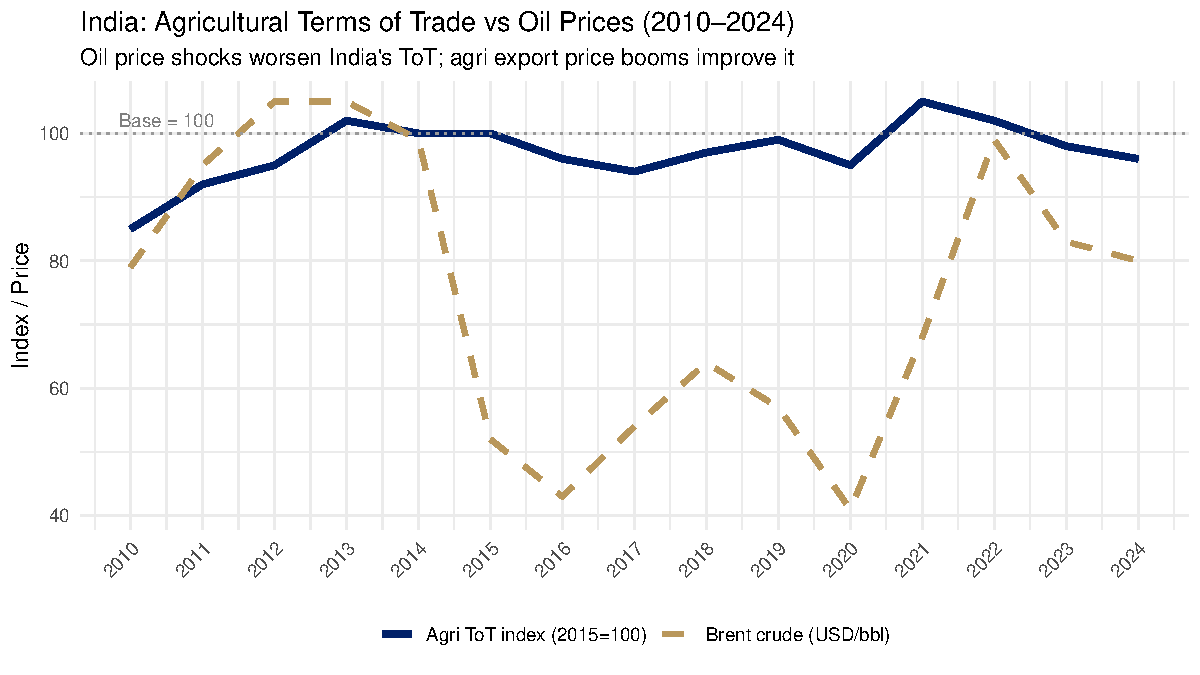
\includegraphics[keepaspectratio]{Lecture06_Terms_of_Trade_files/figure-beamer/fig-india-tot-1.pdf}}

}

\caption{\label{fig-india-tot}India's Commodity Terms of Trade
(Agricultural Exports vs All Imports), 2010--2024 Source: RBI Annual
Report; DGCI\&S.}

\end{figure}%

\textbf{Prebisch-Singer in action:} India's agricultural ToT has broadly
stagnated near or below 100 since 2016 --- consistent with the long-run
deterioration hypothesis. Energy price pass-through via fertilisers and
logistics is the proximate channel.
\end{frame}

\begin{frame}{Prebisch-Singer Hypothesis: Theoretical Foundations}
\phantomsection\label{prebisch-singer-hypothesis-theoretical-foundations}
\begin{columns}[T]
\begin{column}{0.55\linewidth}
\textbf{Raúl Prebisch} (ECLA, 1950) and \textbf{Hans Singer} (UN, 1950)
--- independently:

\begin{quote}
\emph{``The long-run terms of trade of primary commodity exporters
deteriorate relative to manufactures exporters.''}
\end{quote}

Formally, the PS hypothesis states that for primary commodity exporters:

\[\frac{d}{dt}\left(\frac{P_{\text{primary}}}{P_{\text{manufactures}}}\right) < 0 \quad \text{(secular deterioration over time)}\]

Two demand-side forces drive this:

\[\varepsilon_{\text{food}}^{M} < 1 \quad \text{(Engel's Law: income elasticity of food demand} < 1\text{)}\]
\[\varepsilon_{\text{manufactures}}^{M} > 1 \quad \text{(manufactures are income-elastic)}\]

So as world incomes rise, demand for manufactures grows faster than
demand for primary goods, driving down the relative price of primary
commodities.

\textbf{Theoretical reasons:}

\begin{enumerate}
\tightlist
\item
  \textbf{Income elasticity:} Demand for food \textless{} 1 (Engel's
  Law) --- as incomes rise, food share of spending falls
\item
  \textbf{Technological substitutes:} Synthetic rubber replaces natural
  rubber; artificial sweeteners replace sugar
\item
  \textbf{Market power asymmetry:} Northern manufacturers can resist
  wage-price pass-through; Southern commodity prices are competitive
\item
  \textbf{Productivity gains absorbed differently:} In manufactures,
  productivity → lower prices \emph{and} higher wages; in commodities,
  productivity → mainly lower prices
\end{enumerate}
\end{column}

\begin{column}{0.45\linewidth}
\textbf{PS Hypothesis implies:}

Primary commodity exporters should \textbf{diversify} into manufacturing
and high-value processed goods to escape the terms of trade trap.

\[\text{Escape strategy:} \; P_{\text{primary}} \to P_{\text{processed}} \to P_{\text{manufactures}}\]

This is the intellectual foundation for APEDA's mandate: push India up
the value chain.
\end{column}
\end{columns}
\end{frame}

\begin{frame}{Prebisch-Singer: Evidence and India's Experience}
\phantomsection\label{prebisch-singer-evidence-and-indias-experience}
\begin{columns}[T]
\begin{column}{0.55\linewidth}
\textbf{If agricultural ToT decline over time → India must respond:}

\textbf{Strategy 1: Value Addition}

Move from raw commodity exports to processed/packaged exports: - Raw
spices → essential oils, spice powders, branded retail packs - Raw
cotton → yarn → fabric → garments - Fresh fish → frozen fillets →
value-added seafood products

APEDA's (Agricultural and Processed Food Products Export Development
Authority) mandate is exactly this.

\textbf{Strategy 2: High-Value Diversification}

Shift export basket toward: - Basmati rice (premium; RCA
\textasciitilde12) - Organic certified produce (higher prices) -
Floriculture (Netherlands model) - Processed food and beverages
\end{column}

\begin{column}{0.45\linewidth}
\textbf{Evidence:}

The evidence is \emph{contested} but broadly supportive:

\begin{itemize}
\tightlist
\item
  Grilli-Yang (1988) commodity index: secular decline in real commodity
  prices 1900--1987
\item
  Cuddington (1992): decline present but not uniform across commodities
\item
  Post-2000 ``supercycle'' temporarily reversed the trend
\item
  Post-2011: commodity prices fell again
\end{itemize}

\textbf{For India:} Even if the long-run trend is weak,
\emph{volatility} creates serious policy challenges for agricultural
planning.

\textbf{India's Export Composition Shift:}

\begin{longtable}[]{@{}lll@{}}
\toprule\noalign{}
Category & FY2015 share & FY2023 share \\
\midrule\noalign{}
\endhead
Raw cereals & 35\% & 28\% \\
Processed food & 22\% & 31\% \\
Marine (value-added) & 18\% & 22\% \\
Spice derivatives & 8\% & 12\% \\
\bottomrule\noalign{}
\end{longtable}

Trend: India slowly shifting toward value-added exports --- consistent
with the P-S prescription.
\end{column}
\end{columns}
\end{frame}

\section{Part II: Free Trade --- Theory and India's
Reality}\label{part-ii-free-trade-theory-and-indias-reality}

\begin{frame}{The Case for Free Trade}
\phantomsection\label{the-case-for-free-trade}
\begin{columns}[T]
\begin{column}{0.55\linewidth}
\textbf{Standard economic arguments for free trade:}

\begin{enumerate}
\tightlist
\item
  \textbf{Comparative advantage gains} --- world output maximized;
  consumption beyond PPF
\item
  \textbf{Consumer welfare} --- lower prices for imported goods
\item
  \textbf{Economies of scale} --- access to larger markets enables scale
  efficiencies
\item
  \textbf{Technology transfer} --- foreign competition and investment
  bring technology
\item
  \textbf{Competition discipline} --- domestic inefficiency reduced
  under import pressure
\item
  \textbf{Political economy of peace} --- trading partners have
  incentive to maintain peace (Kant's ``perpetual peace'' through
  commerce)
\end{enumerate}

\textbf{Consensus view:} Free trade raises \emph{aggregate} welfare. The
gains to consumers exceed the losses to import-competing producers.
\end{column}

\begin{column}{0.45\linewidth}
\textbf{How strong is the consensus?}

Nobel laureates supporting free trade (qualified): Samuelson, Krugman,
Bhagwati, Sen, Deaton.

But the consensus is increasingly \emph{qualified:} - Distributional
effects matter (Autor, Dorn, Hanson on China shock) - Adjustment costs
are large and concentrated - Market failures (externalities, infant
industries) justify intervention - Agriculture is special: food
security, livelihoods, culture

The debate is not \emph{whether} to trade but \emph{under what
conditions} and \emph{with what safeguards.}
\end{column}
\end{columns}
\end{frame}

\begin{frame}{Economic Arguments for Agricultural Protection}
\phantomsection\label{economic-arguments-for-agricultural-protection}
\begin{columns}[T]
\begin{column}{0.5\linewidth}
\textbf{Economic arguments:}

\begin{enumerate}
\tightlist
\item
  \textbf{Infant industry} --- young industries need protection to
  develop (Hamilton, List, Mill): India's processed food industry
\item
  \textbf{Terms of trade argument} --- large countries can improve ToT
  by taxing exports/imports (optimal tariff)
\item
  \textbf{Revenue argument} --- agricultural tariffs generate government
  revenue
\item
  \textbf{Externalities} --- agriculture provides environmental services
  (biodiversity, groundwater recharge) not priced in markets
\end{enumerate}

\textbf{Agriculture's special status in WTO:}

Agriculture is treated differently: Amber Box (trade-distorting), Blue
Box, Green Box subsidies --- recognizing that pure free trade in
agriculture is politically and socially untenable globally.
\end{column}

\begin{column}{0.5\linewidth}
\textbf{WTO Special Agricultural Status}

The Agreement on Agriculture (AoA, 1995) explicitly recognises
agriculture's special character:

\begin{itemize}
\tightlist
\item
  \textbf{Green Box:} Domestic support that is non- or minimally
  trade-distorting --- exempt from reduction
\item
  \textbf{Blue Box:} Production-limiting support --- exempt
\item
  \textbf{Amber Box:} Trade-distorting support --- must be reduced, but
  not to zero
\item
  \textbf{de minimis provision:} Developing countries may provide up to
  10\% of value of production without counting toward AMS
\end{itemize}

This architecture reflects a consensus that pure free trade in
agriculture would destabilise rural livelihoods and food security in
developing countries.
\end{column}
\end{columns}
\end{frame}

\begin{frame}{Non-Economic and Political Economy Arguments}
\phantomsection\label{non-economic-and-political-economy-arguments}
\begin{columns}[T]
\begin{column}{0.5\linewidth}
\textbf{Non-economic arguments (politically powerful):}

\begin{enumerate}
\setcounter{enumi}{4}
\tightlist
\item
  \textbf{Food security} --- strategic autonomy; cannot depend on
  imports for staple food (India's rice ban logic)
\item
  \textbf{Rural employment} --- 45\% of India's workforce; free trade
  could displace millions
\item
  \textbf{Cultural preservation} --- farming as a way of life, not just
  an industry
\item
  \textbf{Poverty concentration} --- India's poor are mostly in
  agriculture; import competition hits them hardest
\end{enumerate}
\end{column}

\begin{column}{0.5\linewidth}
\textbf{India's Agricultural Tariff Shield}

India applies high bound and applied tariffs on sensitive agricultural
commodities:

\begin{longtable}[]{@{}ll@{}}
\toprule\noalign{}
Commodity & Applied Tariff \\
\midrule\noalign{}
\endhead
Refined palm oil & 100\% \\
Wheat & 50\% \\
Sugar & 100\% \\
Milk powder & 60\% \\
Rice & 100\% (non-Basmati) \\
\bottomrule\noalign{}
\end{longtable}

Average applied agricultural tariff \textasciitilde36\%; bound tariff
\textasciitilde114\%. This large tariff ``water'' gives India policy
space to adjust to domestic supply conditions --- consistent with WTO
rules under the SSM for developing countries.
\end{column}
\end{columns}
\end{frame}

\begin{frame}{India and Free Trade: A Mixed Record}
\phantomsection\label{india-and-free-trade-a-mixed-record}
\textbf{India's Agricultural Trade Policy Stance}

\begin{columns}[T]
\begin{column}{0.5\linewidth}
\textbf{Liberalized:} - Export of rice, wheat, spices, cotton ---
broadly free (with periodic restrictions) - Foreign direct investment in
food processing - Agri commodity futures markets (SEBI regulation) -
Most horticultural exports

\textbf{Protected:} - Edible oils: high tariffs (100\% basic customs
duty on palm oil) - Dairy: SPS barriers and high tariffs - Sugar: export
subsidies + import tariffs - Pulses: periodic import and export
restrictions
\end{column}

\begin{column}{0.5\linewidth}
\textbf{Key Agricultural Tariff Rates (2023):}

\begin{longtable}[]{@{}ll@{}}
\toprule\noalign{}
Commodity & Applied Tariff \\
\midrule\noalign{}
\endhead
Refined palm oil & 100\% \\
Crude palm oil & 100\%* \\
Wheat & 50\% \\
Sugar & 100\% \\
Milk powder & 60\% \\
Rice & 100\% (non-Basmati) \\
\bottomrule\noalign{}
\end{longtable}

*Reduced temporarily in 2022--23 to combat inflation

India uses tariffs \emph{flexibly} --- adjusting to domestic supply
conditions. This is consistent with WTO rules under the SSM (Special
Safeguard Mechanism) for developing countries.
\end{column}
\end{columns}
\end{frame}

\section{Part III: Free Trade
Agreements}\label{part-iii-free-trade-agreements}

\begin{frame}{What is an FTA?}
\phantomsection\label{what-is-an-fta}
\textbf{Levels of Regional Trade Integration (Balassa, 1961)}

\begin{longtable}[]{@{}
  >{\raggedright\arraybackslash}p{(\linewidth - 4\tabcolsep) * \real{0.2414}}
  >{\raggedright\arraybackslash}p{(\linewidth - 4\tabcolsep) * \real{0.4483}}
  >{\raggedright\arraybackslash}p{(\linewidth - 4\tabcolsep) * \real{0.3103}}@{}}
\toprule\noalign{}
\begin{minipage}[b]{\linewidth}\raggedright
Level
\end{minipage} & \begin{minipage}[b]{\linewidth}\raggedright
Description
\end{minipage} & \begin{minipage}[b]{\linewidth}\raggedright
Example
\end{minipage} \\
\midrule\noalign{}
\endhead
\textbf{Preferential Trade Arrangement (PTA)} & Reduced (not zero)
tariffs on selected goods & India-MERCOSUR PTA \\
\textbf{Free Trade Area (FTA)} & Zero tariffs on most goods between
members; each keeps own external tariffs & India-ASEAN FTA \\
\textbf{Customs Union} & FTA + common external tariff & MERCOSUR \\
\textbf{Common Market} & Customs Union + free factor mobility & EU
Single Market (pre-2009) \\
\textbf{Economic Union} & Common Market + harmonized economic policies &
Eurozone \\
\bottomrule\noalign{}
\end{longtable}

India's agreements are mostly \textbf{FTAs} (or ``CEPAs'' ---
Comprehensive Economic Partnership Agreements, which add services and
investment). India has not entered any customs union --- and is unlikely
to, given its strategic autonomy concerns.
\end{frame}

\begin{frame}{India's Major FTAs: An Overview}
\phantomsection\label{indias-major-ftas-an-overview}
\begin{columns}[T]
\begin{column}{0.55\linewidth}
\textbf{India's active FTAs and CEPAs (as of 2025):}

\begin{longtable}[]{@{}llll@{}}
\toprule\noalign{}
Agreement & Year & Type & Key Partners \\
\midrule\noalign{}
\endhead
SAFTA & 2004 & FTA & SAARC nations \\
ASEAN-India (AIFTA) & 2010 & FTA & 10 ASEAN countries \\
India-South Korea CEPA & 2010 & CEPA & South Korea \\
India-Japan CEPA & 2011 & CEPA & Japan \\
India-UAE CEPA & 2022 & CEPA & UAE \\
India-Australia ECTA & 2022 & Interim & Australia \\
\bottomrule\noalign{}
\end{longtable}

\textbf{Under negotiation:} - India-UK FTA (ongoing, 2025) - India-EU
FTA (restarted 2022) - India-Canada (stalled)
\end{column}

\begin{column}{0.45\linewidth}
\textbf{Agricultural market access} is the central sticking point in
every FTA negotiation:

\begin{itemize}
\tightlist
\item
  India is defensive on dairy (EU, Australia, New Zealand pressure)
\item
  India is offensive on rice, spices, mangoes, processed foods
\item
  Developed country partners want India to lower agricultural tariffs
\item
  India resists, citing food security and rural livelihoods
\end{itemize}

The asymmetry: developed country agricultural subsidies (EU CAP, US Farm
Bill) remain intact even as they demand India liberalize.
\end{column}
\end{columns}
\end{frame}

\begin{frame}{India-UAE CEPA (2022): A New Template}
\phantomsection\label{india-uae-cepa-2022-a-new-template}
\begin{columns}[T]
\begin{column}{0.6\linewidth}
\textbf{Background:}

\begin{itemize}
\tightlist
\item
  Signed: February 18, 2022 --- India's first major FTA in a decade
\item
  Entered into force: May 1, 2022
\item
  Full name: India-UAE Comprehensive Economic Partnership Agreement
\end{itemize}

\textbf{Agricultural provisions:}

\begin{itemize}
\tightlist
\item
  UAE granted \textbf{0\% tariff} on 97\% of Indian goods (by tariff
  lines)
\item
  India's key gains: fruits, vegetables, spices, processed food, cereals
\item
  UAE = a re-export hub → India's goods gain access to Gulf, Africa, CIS
\item
  Target: bilateral trade of \textbf{\$100 billion by 2030} (up from
  \$60B in 2021--22)
\end{itemize}

\textbf{Early agricultural results:}

\begin{itemize}
\tightlist
\item
  First 6 months: agri exports to UAE ≈ ₹2,000 crore
\item
  Mango exports to UAE up 40\% in 2022
\item
  Spice exports doubled through UAE gateway
\end{itemize}
\end{column}

\begin{column}{0.4\linewidth}
\textbf{Why the UAE CEPA was easier:}

UAE does NOT have significant agriculture → no defensive interests to
protect.

India could be more aggressive on gaining agri market access.

\textbf{Contrast with EU FTA (stuck):}

EU demands India: - Cut dairy tariffs (protecting French, Dutch dairy) -
Open market for EU wines and spirits - Reduce wheat and sugar tariffs

India cannot concede without political backlash from farmers' lobbies.
\end{column}
\end{columns}
\end{frame}

\begin{frame}{The ASEAN-India FTA: Gains and Losses}
\phantomsection\label{the-asean-india-fta-gains-and-losses}
\begin{columns}[T]
\begin{column}{0.55\linewidth}
\textbf{ASEAN-India Free Trade Agreement in Goods (2010):}

\begin{itemize}
\tightlist
\item
  Covered \textasciitilde80\% of traded goods; zero/reduced tariffs
\item
  India's major concern: agricultural imports from Southeast Asia
\end{itemize}

\textbf{What happened post-2010:}

\textbf{Palm oil imports from Malaysia and Indonesia:} - FY2009: India
imported 6.5 MT palm oil - FY2015: 9.0 MT (38\% increase) - Domestic
edible oil producers devastated

\textbf{Pepper controversy:} - Black pepper imports from Vietnam surged
- Kerala pepper growers (2 million families) badly hurt - Price fell
from ₹800/kg to ₹200/kg at farm gate - Government ultimately raised
duties partially
\end{column}

\begin{column}{0.45\linewidth}
\textbf{The ASEAN FTA Lesson:}

An FTA that looks balanced on paper can have \textbf{asymmetric sectoral
effects} in agriculture.

India's mistake: underestimated: 1. ASEAN agricultural competitiveness
(tropical commodities) 2. Trade diversion effects 3. Adjustment costs
for specific farming communities

\textbf{Corrective action taken:} - 2023: India raised basic customs
duty on edible oils to \textasciitilde100\% despite ASEAN FTA
commitments (using permitted safeguard provisions) - Effective
renegotiation of agricultural elements ongoing
\end{column}
\end{columns}
\end{frame}

\begin{frame}{India's Trade Balance with FTA Partners}
\phantomsection\label{indias-trade-balance-with-fta-partners}
\begin{figure}

\centering{

\pandocbounded{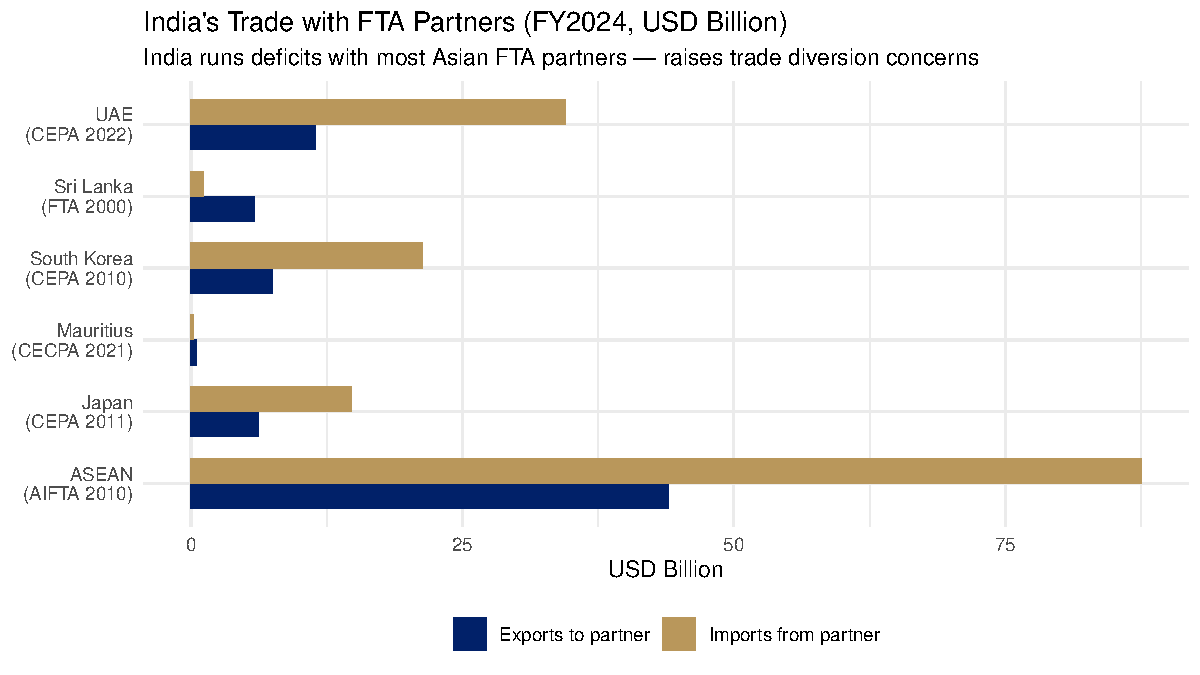
\includegraphics[keepaspectratio]{Lecture06_Terms_of_Trade_files/figure-beamer/fig-india-fta-1.pdf}}

}

\caption{\label{fig-india-fta}India's Trade Balance with Key FTA
Partners (USD billion, FY2024) Source: DGCI\&S / Ministry of Commerce
and Industry, GoI.}

\end{figure}%

\textbf{Trade diversion concern:} India's deficit with ASEAN (\$44B)
deepened \emph{after} the 2010 FTA --- consistent with trade diversion
from efficient global producers to ASEAN partners (particularly palm oil
from Indonesia/Malaysia and electronics from Vietnam).
\end{frame}

\begin{frame}{India and RCEP: The Exit Decision}
\phantomsection\label{india-and-rcep-the-exit-decision}
\begin{columns}[T]
\begin{column}{0.6\linewidth}
\textbf{RCEP --- Regional Comprehensive Economic Partnership:}

\begin{itemize}
\tightlist
\item
  World's largest trade bloc by GDP (\$26.2 trillion, 30\% of global
  GDP)
\item
  Members: 10 ASEAN + China, Japan, South Korea, Australia, New Zealand
\item
  7-year negotiation (2012--2019)
\end{itemize}

\textbf{India walked away on November 4, 2019. Why?}

\begin{enumerate}
\tightlist
\item
  \textbf{China's agricultural flooding:} India feared cheap Chinese
  goods (dairy, fruits, vegetables) would devastate domestic producers
  via zero tariff rules of origin
\item
  \textbf{New Zealand dairy:} NZ dairy exports would destroy India's
  cooperatives (Amul model)
\item
  \textbf{Australian wheat:} Cheap Australian wheat at zero tariff →
  threat to Indian wheat farmers
\item
  \textbf{Services asymmetry:} India wanted labour mobility (IT
  professionals); RCEP offered goods access but not services
\end{enumerate}

PM Modi: \emph{``When I measure the RCEP against the interests of
farmers, MSMEs, and industry, I do not get a positive answer.''}
\end{column}

\begin{column}{0.4\linewidth}
\textbf{Assessment:}

\textbf{Costs of staying out:} - Excluded from the world's largest
trading bloc - Japanese, Korean, ASEAN firms invest in RCEP countries,
not India - India's export competitiveness in RCEP markets weakened

\textbf{Benefits of staying out:} - Protected \textasciitilde150 million
dairy farmers - Protected paddy/wheat cultivators from Australian/NZ
competition - Retained policy space for industrial development

\textbf{Verdict:} The decision reflected India's correct prioritization
of agricultural and rural livelihood protection over trade integration
gains. Whether it was the right long-term decision remains debated.
\end{column}
\end{columns}
\end{frame}

\begin{frame}{Trade Creation vs.~Trade Diversion}
\phantomsection\label{trade-creation-vs.-trade-diversion}
\textbf{Viner's (1950) Framework for Evaluating FTAs}

\begin{columns}[T]
\begin{column}{0.5\linewidth}
\textbf{Trade Creation:}

An FTA creates trade when it shifts consumption from \emph{high-cost
domestic production} to \emph{low-cost partner country production.}

→ \textbf{Efficiency-improving}; welfare-enhancing.

\textbf{Example:} India-UAE CEPA → India imports UAE petrochemicals more
cheaply than domestic production. Cost savings real.
\end{column}

\begin{column}{0.5\linewidth}
\textbf{Trade Diversion:}

An FTA diverts trade when it shifts imports from the \emph{most
efficient world producer} to a \emph{less efficient FTA partner.}

→ \textbf{Efficiency-reducing}; welfare may fall even as trade rises.

\textbf{Example:} If India imports Malaysian palm oil (higher cost)
instead of Indonesian palm oil (lower cost) because of ASEAN FTA tariff
preferences --- trade is \emph{diverted.}
\end{column}
\end{columns}

\textbf{Rule:} An FTA is welfare-improving only if trade \emph{creation}
\textgreater{} trade \emph{diversion}. For India's agricultural FTAs,
the evidence is mixed --- ASEAN FTA likely created significant trade
diversion in edible oils, hurting India's net welfare.
\end{frame}

\begin{frame}{Trade Creation vs.~Trade Diversion: Formal Analysis}
\phantomsection\label{trade-creation-vs.-trade-diversion-formal-analysis}
The net welfare effect of forming an FTA (Viner, 1950):

\[\Delta W_{\text{FTA}} = \underbrace{TC}_{\substack{\text{efficiency gain:}\\ \text{domestic production} \\ \text{→ cheaper partner}}} - \underbrace{TD}_{\substack{\text{efficiency loss:}\\ \text{cheap ROW imports} \\ \text{→ dearer partner}}}\]

\textbf{FTA is welfare-improving if and only if \(TC > TD\).}

Conditions that favour trade creation: 1. Pre-FTA tariffs are
\textbf{high} (larger production distortions to eliminate) 2. Partner is
\textbf{nearly as efficient} as rest-of-world 3. \textbf{High trade
volume} between members (more scope for creation) 4. \textbf{Similar
factor endowments} (complementary comparative advantages)

\begin{figure}

\centering{

\pandocbounded{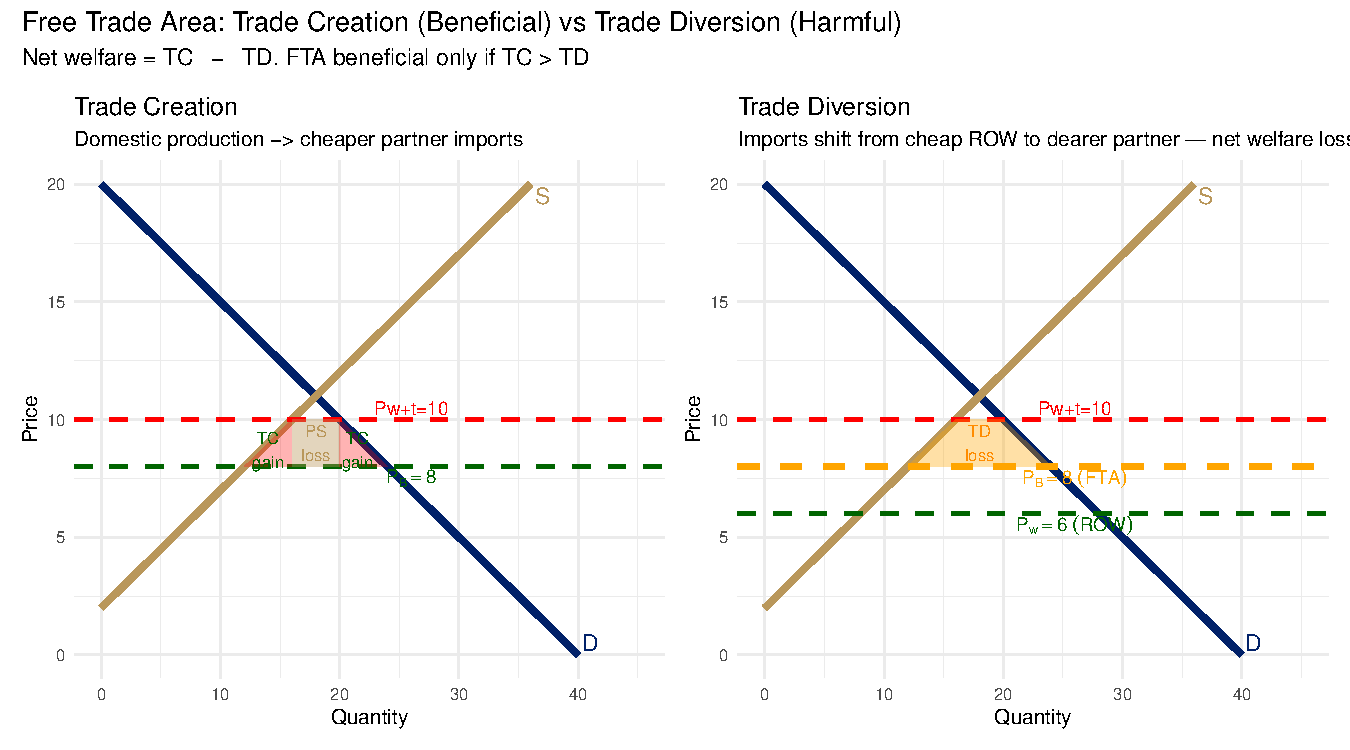
\includegraphics[keepaspectratio]{Lecture06_Terms_of_Trade_files/figure-beamer/fig-trade-creation-1.pdf}}

}

\caption{\label{fig-trade-creation}FTA: Trade Creation (gain, left) vs
Trade Diversion (loss, right) Source: Author's illustration.}

\end{figure}%
\end{frame}

\begin{frame}{Current FTA Negotiations: Key Issues}
\phantomsection\label{current-fta-negotiations-key-issues}
\begin{columns}[T]
\begin{column}{0.55\linewidth}
\textbf{India-UK FTA (under negotiation, 2025):}

\begin{itemize}
\tightlist
\item
  Largest bilateral negotiation since India-UAE
\item
  UK wants: lower Indian tariffs on Scotch whisky, luxury cars,
  financial services
\item
  India wants: UK visa liberalization for IT professionals; lower
  tariffs on textiles, garments, processed food
\item
  \textbf{Agricultural sticking points:} UK dairy access, Indian basmati
  rice in UK market
\end{itemize}

\textbf{India-EU FTA (restarted 2022):}

\begin{itemize}
\tightlist
\item
  Restarted after 8-year gap
\item
  EU demands: dairy market access, geographical indications (GI)
  protection, SPS harmonization
\item
  India demands: visa liberalization, textile market access
\item
  \textbf{Agricultural sticking points:} EU dairy (France, Netherlands),
  EU wines, Indian mango and rice exports
\end{itemize}
\end{column}

\begin{column}{0.45\linewidth}
\textbf{The Common Pattern in All India FTA Negotiations:}

\begin{enumerate}
\tightlist
\item
  \textbf{India is defensive} on dairy, edible oils, wines, processed
  food from developed countries
\item
  \textbf{India is offensive} on rice, spices, garments, IT services
\item
  \textbf{Agricultural market access is always the last issue resolved}
  --- or blocks the deal entirely
\item
  \textbf{The RCEP precedent} haunts all negotiations --- India's
  farmers (and their political representatives) are wary of any deal
  that opens agricultural markets
\end{enumerate}

Agriculture = the political economy constraint binding all India's FTA
negotiations.
\end{column}
\end{columns}
\end{frame}

\begin{frame}{Trade Policy Instruments: A Quick Map}
\phantomsection\label{trade-policy-instruments-a-quick-map}
\textbf{How Countries Restrict Trade (Preview for Lecture 7)}

\begin{columns}[T]
\begin{column}{0.5\linewidth}
\textbf{Tariff instruments:} - Basic customs duty (BCD) - Countervailing
duty (CVD) - Anti-dumping duty (ADD) - Safeguard duty (temporary)

\textbf{Non-tariff barriers:} - Quantitative restrictions (quotas) -
Sanitary and phytosanitary (SPS) measures - Technical barriers to trade
(TBT) - Export subsidies (Amber Box, Blue Box under WTO)
\end{column}

\begin{column}{0.5\linewidth}
\textbf{India's agricultural policy toolkit:}

\begin{itemize}
\tightlist
\item
  \textbf{Export restrictions:} MEP (Minimum Export Price), export bans
\item
  \textbf{Import restrictions:} High tariffs, SPS barriers, MRL (Maximum
  Residue Level) standards
\item
  \textbf{Domestic support:} MSP, PM-KISAN, fertilizer subsidy
\item
  \textbf{Trade facilitation:} APEDA market development, GI tags
\end{itemize}

\textbf{Next lecture (Lecture 7):} Tariffs and quotas in detail ---
their welfare effects, WTO disciplines, and India's use of these
instruments.
\end{column}
\end{columns}

:::
\end{frame}

\begin{frame}{Summary}
\phantomsection\label{summary}
\textbf{Lecture 6 --- Core Concepts}

\begin{enumerate}
\item
  \textbf{Terms of Trade} --- the export-import price ratio; India's
  agricultural ToT is volatile and structurally challenged
\item
  \textbf{Prebisch-Singer Hypothesis} --- primary commodity prices
  decline relative to manufactures over the long run; India must move
  toward value-added exports
\item
  \textbf{Free trade} --- maximizes aggregate welfare through
  comparative advantage, but has distributional consequences;
  agriculture requires special treatment
\item
  \textbf{FTAs} --- second-best instruments driven by political economy;
  trade creation vs.~diversion is the welfare test
\item
  \textbf{India's FTA strategy} --- defensive on agriculture; offensive
  on services and labour-intensive manufactures; RCEP exit reflects
  agricultural protection priorities
\item
  \textbf{India-UAE CEPA} --- India's new template: FTAs with
  non-agricultural partners are easier to conclude
\item
  \textbf{Key negotiating constraint} --- Agricultural market access is
  the binding constraint in all India's major FTA negotiations
\end{enumerate}
\end{frame}

\begin{frame}{Next Lecture: Protectionism --- Tariffs and Quotas}
\phantomsection\label{next-lecture-protectionism-tariffs-and-quotas}
\textbf{Lecture 7 --- June 9, 2026}

\textbf{Instruments of Agricultural Protectionism:}

\begin{enumerate}
\tightlist
\item
  \textbf{Tariffs} --- specific vs.~ad valorem; partial and general
  equilibrium effects; welfare analysis (consumer surplus, producer
  surplus, government revenue)
\item
  \textbf{Quotas} --- tariff-rate quotas (TRQs) in WTO; welfare effects;
  rent seeking
\item
  \textbf{India's tariff structure in agriculture} --- bound vs.~applied
  tariffs; tariff water
\item
  \textbf{Non-tariff barriers} --- SPS standards, MRL limits, labelling
  requirements as instruments of protection
\item
  \textbf{India's edible oil import protection story} --- a case study
  in the political economy of agricultural tariffs
\end{enumerate}

\textbf{Preparation:} Review WTO's Agricultural Agreement (Articles 4--6
on market access) and India's Schedule of Concessions.
\end{frame}

\begin{frame}
\emph{ECO 2203 \textbar{} Department of Agricultural Economics
\textbar{} Lecture 6 of 12}
\end{frame}

\section{Appendix}\label{appendix}

\begin{frame}{Additional Resources}
\phantomsection\label{additional-resources}
\begin{columns}[T]
\begin{column}{0.5\linewidth}
\textbf{Further Reading}

\begin{itemize}
\tightlist
\item
  \emph{International Economics} --- Salvatore (Ch. 7-8)
\item
  \emph{International Economics} --- Appleyard \& Field (Ch. 7-8)
\item
  RBI/DGCI\&S/APEDA databases for latest data
\end{itemize}
\end{column}

\begin{column}{0.5\linewidth}
\textbf{Key Data Sources}

\begin{itemize}
\tightlist
\item
  DGCI\&S: India's merchandise trade
\item
  RBI: Balance of payments data\\
\item
  APEDA: Agricultural export statistics
\item
  WTO: Tariff and trade databases
\end{itemize}
\end{column}
\end{columns}
\end{frame}




\end{document}
